% Modelo desenvolvido por Paulo H O Rodrigues : )
\documentclass[
	% -- opções da classe memoir --
	12pt,					% tamanho da fonte
	openright,				% capítulos começam em pág ímpar (insere página vazia caso preciso)
	oneside,					% para impressão em verso e anverso. Oposto a twoside
	a4paper,					% tamanho do papel. 
	% -- opções da classe abntex2 --
	%chapter=TITLE,			% títulos de capítulos convertidos em letras maiúsculas
	%section=TITLE,			% títulos de seções convertidos em letras maiúsculas
	%subsection=TITLE,		% títulos de subseções convertidos em letras maiúsculas
	%subsubsection=TITLE,	% títulos de subsubseções convertidos em letras maiúsculas
	% -- opções do pacote babel --
	english,					% idioma adicional para hifenização
	%french,					% idioma adicional para hifenização
	%spanish,				% idioma adicional para hifenização
	brazil					% o último idioma é o principal do documento
	]{abntex2}

% ---------------------
% Pacotes OBRIGATÓRIOS
% ---------------------
\usepackage{lmodern}				% Usa a fonte Latin Modern			
\usepackage[T1]{fontenc}			% Selecao de codigos de fonte.
\usepackage[utf8]{inputenc}		% Codificacao do documento (conversão automática dos acentos)
\usepackage{lastpage}			% Usado pela Ficha catalográfica
\usepackage{indentfirst}		% Indenta o primeiro parágrafo de cada seção.
\usepackage{color}				% Controle das cores
\usepackage{graphicx,graphicx}	% Inclusão de gráficos
\usepackage{epsfig,subfig}		% Inclusão de figuras
\captionsetup[figure]{labelfont={bf},name={Fig.},labelsep=period} %Altera o nome da figura para texto predefinido
\usepackage{microtype} 			% Melhorias de justificação
% ---------------------
		
% ---------------------
% Pacotes ADICIONAIS
% ---------------------
\usepackage{lipsum}						% Geração de dummy text
\usepackage{amsmath,amssymb,mathrsfs}	% Comandos matemáticos avançados 
\usepackage{setspace}  					% Para permitir espaçamento simples, 1 1/2 e duplo
\usepackage{verbatim}					% Para poder usar o ambiente "comment"
\usepackage{tabularx} 					% Para poder ter tabelas com colunas de largura auto-ajustável
\usepackage{afterpage} 					% Para executar um comando depois do fim da página corrente
\usepackage{url} 						% Para formatar URLs (endereços da Web)
% ---------------------

% ---------------------
% Pacotes de CITAÇÕES
% ---------------------
%\usepackage[brazilian,hyperpageref]{backref}	% Paginas com as citações na bibl
\usepackage[numbers,sort&compress]{natbib} 
%\usepackage[num]{abntex2cite}				% Citações padrão ABNT 
%\usepackage[alf]{abntex2cite}				% Citações padrão ABNT(autor-data)

%Tipo de simbolo
%\citebrackets[] 							 
%\citebrackets()
%\citebrackets{}

% ---------------------

% Configurações de CITAÇÕES para abntex2
%% --- 
% CONFIGURAÇÕES DE PACOTES
% --- 

% ---
% Configurações do pacote backref
% Usado sem a opção hyperpageref de backref
\renewcommand{\backrefpagesname}{Citado na(s) página(s):~}
% Texto padrão antes do número das páginas
\renewcommand{\backref}{}
% Define os textos da citação
\renewcommand*{\backrefalt}[4]{
	\ifcase #1 %
		Nenhuma citação no texto.%
	\or
		Citado na página #2.%
	\else
		Citado #1 vezes nas páginas #2.%
	\fi}%
% ---

% Inclusão de dados para CAPA e FOLHA DE ROSTO (título, autor, orientador, etc.)
\include{pretextual/ContraCapa}

% Inclui Configurações de aparência do PDF Final
%  Configurações de aparência do PDF final
% NÃO ALTERAR!!!

% alterando o aspecto da cor azul
\definecolor{blue}{RGB}{41,5,195}

% informações do PDF
\makeatletter
\hypersetup{
     	%pagebackref=true,
		pdftitle={\@title}, 
		pdfauthor={\@author},
    	pdfsubject={\imprimirpreambulo},
	    pdfcreator={LaTeX with abnTeX2},
		pdfkeywords={abnt}{latex}{abntex}{abntex2}{trabalho acadêmico}, 
		colorlinks=true,       		% false: boxed links; true: colored links
    	linkcolor=blue,          	% color of internal links
    	citecolor=blue,        		% color of links to bibliography
    	filecolor=magenta,      		% color of file links
		urlcolor=blue,
		bookmarksdepth=4
} 
\makeatother
% --- 

% O tamanho da identação do parágrafo é dado por:
\setlength{\parindent}{1.3cm}

% Controle do espaçamento entre um parágrafo e outro:
\setlength{\parskip}{0.2cm}  % tente também \onelineskip

% ---------------------
% Compila o indice
% ---------------------
\makeindex
% ---------------------

%%%%%%%%%%%%%%%%%%%%%%%%%%%
%%  INICIO DO DOCUMENTO  %%
%%%%%%%%%%%%%%%%%%%%%%%%%%%
\begin{document}

% Retira espaço extra obsoleto entre as frases.
\frenchspacing

% ----------------------------------------------------------
% ELEMENTOS PRÉ-TEXTUAIS (Capa, Resumo, Abstract, etc.)
% ----------------------------------------------------------
\pretextual

% Capa
% ---
% Impressão da Capa
% ---
\begin{capa}%
    \begin{center}
    	\begin{figure}[!htb]
    		%Logo GCOM
            
\includegraphics[scale=0.07]{imagens/unipac.jpg} 
    		\hfill
        		\begin{minipage}{10cm} \vskip -3cm
        		\ABNTEXchapterfont\large\center{Fundação Presidente Antônio Carlos\\ Conselheiro Lafaiete \\ Engenharia de Computação}
                \end{minipage}
    		% Logo da engenharia
    		
\includegraphics[scale=0.85]{imagens/eng.jpg}
    	\end{figure}
    \end{center}
    \center
	%\vspace{1.5cm}

    \vfill
    \ABNTEXchapterfont\bfseries\LARGE\imprimirtitulo
    \vfill

	%\vfill
	\ABNTEXchapterfont\large\imprimirautor
	\vfill
%
    \large\imprimirlocal, \large\imprimirdata

    \vspace*{1cm}
 \end{capa}
% ---

% Folha de rosto (o * indica que haverá a ficha bibliográfica)
\imprimirfolhaderosto*

% Imprimir Ficha Catalografica
%% ---
% Ficha Catalográfica
% ---
% Isto é um exemplo de Ficha Catalográfica, ou ``Dados internacionais de
% catalogação-na-publicação''. Você pode utilizar este modelo como referência. 
% Porém, provavelmente a biblioteca da sua universidade lhe fornecerá um PDF
% com a ficha catalográfica definitiva após a defesa do trabalho. Quando estiver
% com o documento, salve-o como PDF no diretório do seu projeto e substitua todo
% o conteúdo de implementação deste arquivo pelo comando abaixo:
%
% \begin{fichacatalografica}
%     \includepdf{fig_ficha_catalografica.pdf}
% \end{fichacatalografica}
\begin{fichacatalografica}
	\vspace*{\fill}					% Posição vertical
	\hrule							% Linha horizontal
	\begin{center}					% Minipage Centralizado
	\begin{minipage}[c]{12.5cm}		% Largura
	
	\imprimirautor
	
	\hspace{0.5cm} \imprimirtitulo  / \imprimirautor. --
	\imprimirlocal, \imprimirdata-
	
	\hspace{0.5cm} \pageref{LastPage} p. : il. (algumas color.) ; 30 cm.\\
	
	\hspace{0.5cm} \imprimirorientadorRotulo~\imprimirorientador\\
	
	\hspace{0.5cm}
	\parbox[t]{\textwidth}{\imprimirtipotrabalho~--~\imprimirinstituicao,
	\imprimirdata.}\\
	
	\hspace{0.5cm}
		1. Palavra-chave1.
		2. Palavra-chave2.
		I. Orientador.
		II. Universidade xxx.
		III. Faculdade de xxx.
		IV. Título\\ 			
	
	\hspace{8.75cm} CDU 02:141:005.7\\
	
	\end{minipage}
	\end{center}
	\hrule
\end{fichacatalografica}
% ---

% Inserir Folha de Aprovação
%% ---
% Assinaturas
% ---
% Isto é um exemplo de Folha de aprovação, elemento obrigatório da NBR
% 14724/2011 (seção 4.2.1.3). Você pode utilizar este modelo até a aprovação
% do trabalho. Após isso, substitua todo o conteúdo deste arquivo por uma
% imagem da página assinada pela banca com o comando abaixo:
%
% \includepdf{folhadeaprovacao_final.pdf}
%
\begin{folhadeaprovacao}

  \begin{center}
    {\ABNTEXchapterfont\large\imprimirautor}

    \vspace*{\fill}\vspace*{\fill}
    \begin{center}
      \ABNTEXchapterfont\bfseries\Large\imprimirtitulo
    \end{center}
    \vspace*{\fill}
    
    \hspace{.45\textwidth}
    \begin{minipage}{.5\textwidth}
        \imprimirpreambulo
    \end{minipage}%
    \vspace*{\fill}
   \end{center}
        
   Trabalho aprovado. \imprimirlocal, XX de XXXX de 202X:

   \assinatura{\textbf{\imprimirorientador} \\ Orientador} 
   \assinatura{\textbf{\imprimircoorientador} \\ Co-Orientador} 
   \assinatura{\textbf{Professor} \\ Convidado 1}
   \assinatura{\textbf{Professor} \\ Convidado 2}
   \assinatura{\textbf{Professor} \\ Convidado 3}
      
   \begin{center}
    \vspace*{0.5cm}
    {\large\imprimirlocal}
    \par
    {\large\imprimirdata}
    \vspace*{1cm}
  \end{center}
  
\end{folhadeaprovacao}
% ---

% Dedicatória
%% ---
% Dedicatória
% ---
\begin{dedicatoria}
   \vspace*{\fill}
   \centering
   \noindent
   \textit{ Aos meus pais XXXXXXXX e YYYYYYY, \\ por sempre estarem comigo em todos os momentos.} \vspace*{\fill}
\end{dedicatoria}
% ---

% Agradecimentos
% ---
% Agradecimentos
% ---
\begin{agradecimentos}

Agradeço a Deus por me iluminar nos momentos difíceis, dando força na longa caminhada.

Em especial minha esposa, por me apoiar incondicionalmente e por sempre confiar em meu potencial me incentivando a fazer sempre o melhor e a meu filho pelas risadas calorosas que me renovam sempre o ânimo e me lembram dos meus objetivos.

%Aos meus irmãos, por.....

Ao meu orientador Alex Vitorino por sua paciência e sempre propondo novos desafios que são de grande contribuição em relação ao meu aprendizado e com ensinamentos importantes para consolidação deste trabalho.

%Aos meus amigos ...

%Aos professores ...

%À XXXXXX pelo apoio financeiro para realização deste trabalho de pesquisa.

Enfim em todos que acreditaram no meu sonho.

\end{agradecimentos}
%% ---

% Epígrafe
% ---
% Epígrafe
% ---
\begin{epigrafe}
    \vspace*{\fill}
	\begin{flushright}
		\textit{``A mão queimada ensina melhor. \\
		          Depois disso o conselho sobre o fogo \\
                  chega ao coração.''-- Gandalf - O Cinzento \\
		          (J.R.R. Tolkien)}
	\end{flushright}
\end{epigrafe}
% ---

% Resumo e Abstract
% ---
% RESUMOS
% ---

% RESUMO em português
\setlength{\absparsep}{18pt} % ajusta o espaçamento dos parágrafos do resumo
\begin{resumo}
    O objetivo deste presente trabalho é a consolidação dos conhecimentos adquiridos durante a realização da disciplina de Sistemas Operacionais, dando enfoque aos sistemas baseados em Linux utilizados em servidores, salientando suas utilizações e o seu mercado de atuação. \\
    O Linux é um sistema operacional que vive em um crescimento contínuo e é amplamente usado ele está tanto em sensores a supercomputadores, e podemos vê-lo sendo usados em espaçonaves, automóveis, \emph{smartphones}, relógios e muitos outros dispositivos em nossa vida cotidiana \cite{LinuxFundationWIL}.\\
    Em especial o sistema Linux é um sistema de código aberto o que significa que é possível executá-lo para qualquer propósito, estudar seu funcionamento e modificá-lo se assim desejar, ou realizar cópias para terceiros dando total liberdade para sua comunidade \cite{LinuxFundationWIL},\cite{Morimoto2011}.\\
    Ele também opera a maior parte da Internet, todos os 500 maiores supercomputadores do mundo e as bolsas de valores do mundo. Estes funcionam em uma variação do Linux preparada para um grande fluxo de tratamento de dados, podendo rodar vários serviços simultaneamente, esta versão é a Linux para servidores ou \emph{Linux Server} \cite{LinuxFundationWIL},\cite{Morimoto2011}.\\





 \textbf{Palavras-chaves}: Linux, Servidores, Sistema Operacional.
\end{resumo}

% ABSTRACT in english
% \begin{resumo}[Abstract]
%  \begin{otherlanguage*}{english}
%   This is the english abstract.

%   \vspace{\onelineskip}
 
%   \noindent 
%   \textbf{Keywords}: latex. abntex. text editoration.
%  \end{otherlanguage*}
% \end{resumo}

% Lista de ilustrações
\pdfbookmark[0]{\listfigurename}{lof}
\listoffigures*
\cleardoublepage

% Lista de tabelas
% \pdfbookmark[0]{\listtablename}{lot}
% \listoftables*
% \cleardoublepage

% Lista de abreviaturas e siglas
\begin{siglas}
    \item[E/S] Entrada e saída
    \item[FreeBSD] Free OS descended from the 
    Berkeley Software Distribution 
    \item[GNU] GNU's Not Unix
    \item[GNU GPL] GNU General Public License
    \item[GUI] Graphical User Interface
    \item[MIT] Massachusetts Institute of Technology
    \item[MULTICS] MULTiplexed Information and Computing Service 
    \item[OS] Operating System  
    \item[OS X] Operating Systems number 10 
    \item[PC] Personal Computer
    \item[SO] Sistema Operacional
\end{siglas}

% Lista de símbolos
%\begin{simbolos}
  \item[$ \Gamma $] Letra grega Gama
  \item[$ \Lambda $] Lambda
  \item[$ \zeta $] Letra grega minúscula zeta
  \item[$ \in $] Pertence
\end{simbolos}

% Inserir o SUMÁRIO
\pdfbookmark[0]{\contentsname}{toc}
\tableofcontents*
\cleardoublepage

% ----------------------------------------------------------
% ELEMENTOS TEXTUAIS (Capítulos)
% ----------------------------------------------------------
\textual
% Elementos textuais com numeração arábica
\pagenumbering{arabic}%arabic
% Reinicia a contagem do número de páginas
\setcounter{page}{1}

% Inclui cada capitulo da Dissertação
% ----------------------------------------------------------
% Introdução 
% Capítulo sem numeração, mas presente no Sumário
% ----------------------------------------------------------

\chapter[Introdução]{Introdução}
%\addcontentsline{toc}{chapter}{Introdução}

Um computador moderno consiste em um emaranhado de peças que contém um ou mais processadores, alguma memória principal, alguma memória secundaria, interfaces de rede diversos periféricos como impressoras, teclado, mouse, monitor e vários outros dispositivos de entrada e saída. Podemos dizer que este é um sistema complexo, para realizar a desafiadora maratona que é compreender como cada parte funciona e gerenciar com maestria esses componentes é um grande desafio \cite{Tanenbaum2016}.\\
Para isso os computadores modernos são equipados com um SO esse dispositivo de \emph{software} tem a função de fornecer uma plataforma simples e limpa para o usuário de forma a ajuda-lo nas entradas e saídas de dados. Em uma visão simplista podemos ver na figura \ref{fig:figura1} onde o SO se encontra em relação entre \emph{hardware} e o usuário \cite{Tanenbaum2016}. 

\begin{figure}[htpb]
    \centering
   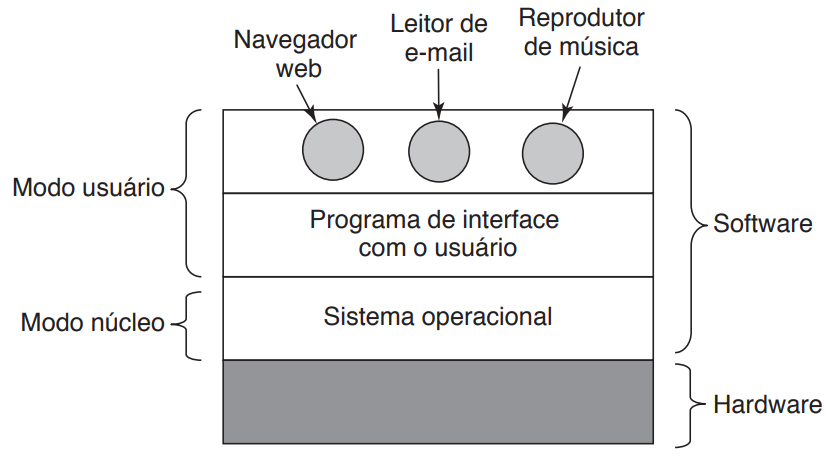
\includegraphics[scale=.4]{imagens/figura1.png}
   \caption{Onde o sistema operacional se encaixa. \cite{Tanenbaum2016}}
   \label{fig:figura1}
\end{figure}

Inicialmente a ideia que temos de um SO é a visão que temos dos ditos sistemas operativos que temos conhecimento que podem ser \emph{Windows}, \emph{Linux}, \emph{FreeBSD}, ou \emph{OS X} mas normalmente a forma de interagir com diretamente com o sistema é através de terminais comumente conhecidos como shell (interpretadores de comando) isto quando baseado em texto ou \emph{GUI (Graphical User Interface)} quando em modo gráfico \cite{Tanenbaum2016}.\\
Um sistema operacional é projetado para ocultar as particularidades de \emph{hardware} (ditas "de baixo nível") e assim criar uma máquina abstrata que fornece às aplicações serviços compreensíveis ao usuário (ditas "de alto nível") \cite{Comer2012}.\\
Assim o sistema trabalha em dois estados o modo núcleo e o modo usuário. Sendo que no modo núcleo (também chamado modo supervisor ou \emph{Kernel mode}). O sistema tem acesso completo aos recursos seja de ao \emph{hardware} ou \emph{software} e pode executar qualquer instrução que a máquina for capaz de executar \cite{Tanenbaum2016}, \cite{linfo2007}.\\
Quando o sistema está em modo \emph{kernel} é considerado que as execuções são de uma fonte confiável e, portanto, pode executar quaisquer instruções e fazer referência a quaisquer endereços de memória (ou seja, locais na memória). O \emph{kernel} tem total controle sobre o sistema e trata todos os outros \emph{software}s como programas não confiáveis, assim todas as operações em modo usuário que necessitem alterar o sistema solicitam ao uso do \emph{kernel} por meio de uma chamada de sistema  para executar instruções privilegiadas, como criação de processos ou operações de entrada / saída \cite{Tanenbaum2016}, \cite{linfo2007}.\\

Neste trabalho iremos trabalhar com o sistemas baseados em \emph{Linux} para servidores mas é importante entender um pouco da evolução desse sistema.

Em meados da década de 60 uma iniciativa conjunta do \emph{MIT}, da \emph{Bell Labs}  e da \emph{General Electric} decidiram embarcar no desenvolvimento de um “computador utilitário”, isto é, uma máquina que daria suporte a algumas centenas de usuários simultâneos em pouco tempo nasce o projeto MULTICS (Serviço de Computação e Informação Multiplexada) \cite{Tanenbaum2016}.\\
O MULTICS foi projetado para ser um sucesso com suporte para centenas de usuários em uma máquina apenas um pouco mais poderosa do que um PC baseado no 386 da \emph{Intel}. Mas transformá lo em um produto final de fácil comercialização não foi amarga realidade \cite{Tanenbaum2016}.\\
A \emph{Bell Labs} abandonou o projeto, e a \emph{General Electric} abandonou completamente o negócio dos computadores. Entretanto, o \emph{MIT} persistiu e finalmente colocou o MULTICS para funcionar.E foi instalado por mais ou menos 80 empresas e universidades importantes mundo afora \cite{Tanenbaum2016}.\\
Um dos cientistas da \emph{Bell Labs} que havia trabalhado no projeto MULTICS, Ken Thompson, decidiu escrever uma versão despojada e para um usuário do MULTICS. Esse trabalho mais tarde desenvolveu-se no sistema operacional UNIX, que se tornou popular no mundo acadêmico, em agências do governo e em muitas empresas \cite{Tanenbaum2016}.\\
Em 1987, Andrew Tanenbaum lançou um pequeno clone do UNIX, chamado MINIX, para fins educacionais. Em termos funcionais, o MINIX é muito similar ao UNIX \cite{Tanenbaum2016}.\\
Em 1991 Linus Torvalds começou um projeto inicialmente um emulador de terminal que era utilizado para acessar os servidores em UNIX da universidade Helsinki. Ele escreveu o código para especificamente  para o \emph{hardware} que utilizava um computador com um processador 80386 ele realizou o desenvolvimento no minix usando o \emph{GNU C compiler} \cite{Torvalds1991}, \cite{Torvalds1993}, \cite{torvalds2002}.\\
O \emph{Linux} também é distribuído sob uma licença de código aberto. O código aberto segue estes locatários principais:
\begin{itemize}
    \item A liberdade de executar o programa, para qualquer propósito.
    \item A liberdade de estudar como o programa funciona e alterá-lo para que ele faça o que você deseja.
    \item A liberdade de redistribuir cópias para que você possa ajudar seu vizinho.
    \item A liberdade de distribuir cópias de suas versões modificadas para terceiros.
\end{itemize}
Esses pontos são cruciais para entender a ideia por trás do \emph{Linux}. O \emph{Linux} se transformou em um sistema de fácil acesso. Com a grande liberdade de se poder modificar o sistema ele proporcionou a criação de diversas distribuições uma vez que qualquer usuário pode criar uma que atenda a suas necessidades \cite{LinuxFundationWIL}.\\
Nos próximos sessões  iremos discutir sobre o sistema e aprofundar no \emph{Linux} para assim entender, suas funcionalidade, modo de funcionamento e  quais suas principais atuações.\\









%\section*{Figuras}\label{sec:figuras}
%\addcontentsline{toc}{section}{figuras}

% \section*{Tabelas}\label{sec:tabelas}
% \addcontentsline{toc}{section}{tabelas}

%\section*{Motivação}\label{sec:motivacao}
%\addcontentsline{toc}{section}{Motivação}

%\section*{Objetivos}\label{sec:objetivos}
%\addcontentsline{toc}{section}{Objetivos}




\section{Revisão sobre hardware de
computadores}
%\addcontentsline{toc}{section}{Estrutura de hardware}
\subsection{Processadores}
A \emph{CPU} (\emph{Central Process Unit} -  no portugues Unidade Central de Processamento) muitas vezes é considerado o cérebro do computador ela é responsável por receber as instruções da memória e processá las, decodificando-as e executando todos os processos em fila de execução num ciclo que é repetido até que o programa termine \cite{Tanenbaum2016}. \\
Assim os programas são executados. Cada \emph{CPU} é presa a sua arquitetura assim não conseguindo decodificar instruções de arquiteturas diferentes como \emph{ARM} para X86 ou vice e versa. A velocidade de cálculo das \emph{CPU`s} é muito maior que o tempo para executar uma instrução registradores internos são utilizados para armazenamento de variáveis e resultados temporários \cite{Tanenbaum2016}.\\
O SO deve conhecer absolutamente todos os processos destinados ao processador e também todos os registradores gerados pois quando a \emph{CPU} realiza uma multiplexação ela interrompe o programa em execução para recomeçar outro. Assim faz-se necessário que o SO tem que salvar todos os registradores de maneira que eles possam ser restaurados quando o programa for executado mais tarde. Muitas \emph{CPU`s} modernas têm recursos para executar mais de uma instrução ao mesmo tempo \cite{Tanenbaum2016}. \\
Por exemplo, uma \emph{CPU} pode ter unidades de busca, decodificação e execução separadas, assim enquanto ela está executando a instrução não, poderia também estar decodificando a instrução n + 1 e buscando a instrução n + 2. Uma organização com essas características é chamada de \emph{pipeline} como na figura \ref{fig:Processador1} abaixo \cite{Tanenbaum2016}.\\
\begin{figure}[htpb]
    \centering
   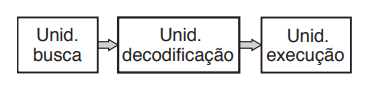
\includegraphics[scale=1]{imagens/Processador1.png}
   \caption{Um \emph{pipeline} com três estágios. \cite{Tanenbaum2016}}
   \label{fig:Processador1}
\end{figure}\\

Ainda mais avançada que um projeto de \emph{\emph{pipeline}} é uma \emph{CPU} superescalar, mostrada na Figura \ref{fig:Processador2}. Nesse projeto, unidades múltiplas de execução estão presentes. Uma unidade para aritmética de números inteiros, por exemplo, uma unidade para aritmética de ponto flutuante e uma para operações booleanas. Duas ou mais instruções são buscadas ao mesmo tempo, decodificadas e jogadas em um \emph{buffer} de instrução até que possam ser executadas. Tão logo uma unidade de execução fica disponível, ela procura no buffer de instrução para ver se há uma instrução que ela pode executar e, se assim for, ela remove a instrução do \emph{buffer} e a executa \cite{Tanenbaum2016}. 
\begin{figure}[htpb]
    \centering
   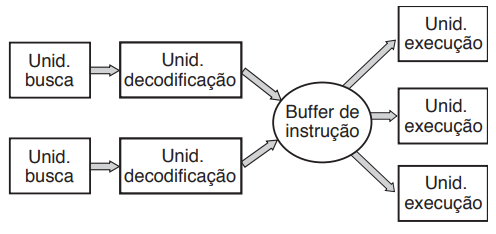
\includegraphics[scale=1]{imagens/Processador2.png}
   \caption{Uma \emph{CPU} superescalar. \cite{Tanenbaum2016}}
   \label{fig:Processador2}
\end{figure}\\

Um \emph{thread} é um tipo de processo leve, mais para o SO cada \emph{thread} é como uma \emph{CPU} separada, considere um sistema com duas \emph{CPU`s} efetivas, cada uma com dois threads. O sistema operacional verá isso como quatro \emph{CPU`s} chamamos isso de \emph{multithreading} \cite{Tanenbaum2016}.
\subsection{Memória}
\subsection{Discos rígidos}
\label{subsection:Discos}
Os discos rígidos mais popularmente conhecidos como HD \emph{(Hard Disk)} é o método mais utilizado para armazenamento de dados pelo computador. utilizando-se de braços metálicos posicionados acima de um disco metálico este gera um pulso eletro magnético para gravar a informação no prato metálico em formato de disco. Tecnologia de desenvolvida em 1956 contava apenas com 5 megabytes de tamanho de armazenamento hoje existem discos com capacidade de armazenamento maior que 10 terabytes \cite{Tanenbaum2016}, \cite{Comer2012}.\\
Normalmente o sistema operacional é gravado  neste disco por ele não ser volátil, ou seja não se apaga mesmo quando o computador está desligado \cite{Tanenbaum2016}, \cite{Comer2012}.
\begin{figure}[htpb]
    \centering
   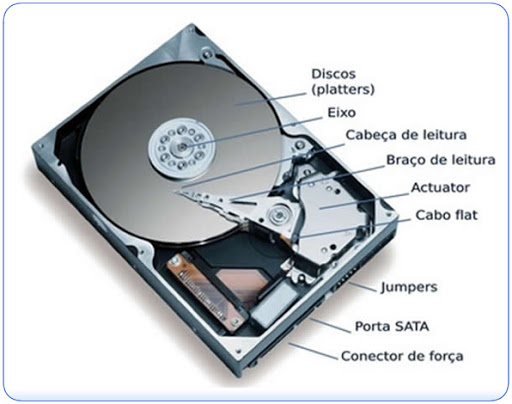
\includegraphics[scale=0.5]{imagens/disco.jpg}
   \caption{Visão de um disco rigido.}
   \label{fig:disco}
\end{figure}
\subsection{Dispositivos de E/S}
O sistema operacional não trabalha apenas com CPU e memórias ele tem que gerenciar outros tipos de hardware estes equipamentos em questão tem funções específicas mas basicamente ele trabalham fazendo o \emph{input} e \emph{output} de informações no sistema e são conhecidos como dispositivos de E/S. podemos dizer que estes dispositivos possuem duas características básicas um controlador e o dispositivo em si \cite{Tanenbaum2016}, \cite{Comer2012}.\\
O controlador ele proporciona a comunicação entre o SO e o dispositivo em si, como cada dispositivo possui características particulares que podem ser influenciadas pelo fabricante ou tecnologia empregada assim se faz necessário que seja disponibilizado para o sistema \emph{software} auxiliares que ajudam o SO a comunicar com o controlador esse \emph{software} são chamados de Drivers \cite{Tanenbaum2016}, \cite{Comer2012}.\\
O dispositivo em si normalmente possui padronização de saídas físicas para que as conexões com o computador sejam simplificadas e por exemplo que uma saída sata seja idêntica independente do fabricante ou da tecnologia empregada para a construção do dispositivo \cite{Tanenbaum2016}, \cite{Comer2012}.
\subsection{Barramentos}
asd
% \subsection{Inicializando o computador}\\

\chapter[Sistema Operacional]{Sistema Operacional}
%\addcontentsline{toc}{chapter}{Sistema Operacional}

Mas afinal o que é um sistema operacional?

É difícil entender o que é um sistema operacional pois talvez a única coisa que podemos afirmar é que é um \emph{software} que trabalhe em modo núcleo (e por vezes até isso não é uma completa verdade), para tal precisamos entender que o SO tem duas funções bases que é fornecer uma abstração do \emph{hardware} para programadores de aplicativos e usuários em geral, e o gerenciamento dos recursos de \emph{hardware}.\\
 Em geral o conjunto de instruções, estrutura de barramento, E/S e a organização de memória é complexo e varia dependendo da arquitetura das peças utilizadas no computador. Por esse motivo o SO fornece uma camada de abstração para os aplicativos que se utilizam dos \emph{hardwares} do computador possam criar, escrever e ler arquivos, sem ter de lidar com os detalhes complexos de como o \emph{hardware} realmente funciona.\\
Como dito anteriormente um computador moderno consiste em um emaranhado de peça e a função do sistema operacional é fornecer uma alocação ordenada e controlada para todas elas além que o SO moderno permite que múltiplas aplicações estejam em memória e sejam executados “ao mesmo tempo”. \\
Precisamos entender que o sistema não faz  execução de todos os recursos ao mesmo tempo isso seria insano de se imaginar mais ele utiliza de filas de processos e de um nivelamento de urgências para definir o que será processado e quando será processado, ele ainda define as utilizações em nível de memória para definir prioridades e utilizando delas para alterar o tempo  de acesso ao processador, desta forma mesmo com vários processos “abertos” a execução se dá em filas multiplexadas \cite{Tanenbaum2016}, \cite{Comer2012}.\\
Ainda devemos entender que se o sistema possuir vários usuários a necessidade de gerenciar e proteger a memória, dispositivos de E/S e outros recursos é ainda maior, pois cada usuário precisa ter acesso aos recursos de \emph{hardwares} e compartilhar de informações salvas como (arquivos, bancos de dados etc.) e as ações de um usuário pode influenciar ao uso do outro \cite{Tanenbaum2016}, \cite{Comer2012}.\\
Podemos dizer então que a função primordial do SO é manter controle, isso seja sobre como conceder acesso a recursos requisitados, sobre quais programas estão usando qual recurso, sobre como conceder recursos requisitados, contabilizar o seu uso, assim como mediar requisições conflitantes de diferentes programas e usuários \cite{Tanenbaum2016}, \cite{Comer2012}.\\
O termo \emph{hardware} foi muito utilizado mais qual seriam os \emph{hardwares} de um computador ou uma estrutura basica dos mesmos e como o sistema operacional se utiliza deles para em sua execução \cite{Tanenbaum2016}, \cite{Comer2012}.



% \section{Estrutura de sistemas operacionais}
asd

\include{capitulos/SecoesSO/OZoológicoDosOSs}

\chapter{Processos e threads}\label{cap:ProcessosThreads}



\section{Processos}\label{sec:Processos}
%\addcontentsline{toc}{section}{Trabalhos Relacionados a Isto}
\section{Threads}\label{sec:Threads}

\section{Comunicação entre processos}\label{sec:ComProc}

\section{Escalonamento}\label{sec:Escalonamento}

\chapter{Gerenciamento de memória}\label{cap:GerenciamentoMemoria}

O processador apesar de sua grande velocidade não consegue armazenar dados logo para que seja possível a execução dos programas pode se dizer que todo computador deve possuir algum tipo de memória.
Podemos dizer que a memória é um grande vetor de palavras ou bytes de variados tamanhos sendo que cada um possui seu próprio endereço. A memória principal é um repositório de dados acessíveis e compartilhados pela \emph{CPU} e dispositivos de entrada/saída \cite{ufscar2019}.\\
Inicialmente os computadores não faziam abstração da memória tendo que realizar a leitura direto da memória física, este tipo de abordagem além de lenta transforma a memória apenas em um grande índice que vai de 0 ao tamanho máximo de endereços da memória fazendo que a informação seja movida de célula a célula de 8 \emph{bits}. Nesta condição quando mais programas forem executado simultaneamente pode ocorre erros sofridos quando um programa apagar os dados salvos por outro \cite{ufscar2019}, \cite{silberschatz2000}, \cite{stallings2004}.\\
Apesar disto é possível que se execute mais de um programa simultaneamente e de forma funcional, desde que exista apenas um programa de cada acessando a memória, para que não exista conflitos. O conceito \emph{swapping} faz com que um sistema operacional salve o conteúdo inteiro da memória em um arquivo de disco assim existe um backup da informação \cite{Tanenbaum2016}.\\
Mas a maioria dos computadores possuem uma hierarquia de que como já visto na figura \ref{fig:lvlmemoria} podemos afirmar ainda que quanto mais longe do processador maior a memória e menor é o seu valor.
No \emph{Linux}, tratamento da memória se dá de forma subdividida, ele trabalha seu gerenciamento com dois componentes: o primeiro, responsável pela alocação e liberação de memória física (páginas, grupos de páginas e pequenos blocos de memória) e o segundo pela memória virtual \cite{ufscar2019}, \cite{silberschatz2000}, \cite{stallings2004}.

\section{Gerência de memória física}

Através de algoritmos como o \emph{Buddy-heap} que rastreiam as páginas físicas disponíveis, o gerente primário de memória física consegue realizar as tarefas ao qual é responsável como alocação e liberação de todas as páginas físicas e é capaz de disponibilizar intervalos de páginas fisicamente contíguas sob demanda. Este tipo de solução trabalha dividindo a memória em partições para tentar satisfazer as requisições de forma adequada \cite{ufscar2019}, \cite{silberschatz2000}, \cite{stallings2004}.\\
Quando se utiliza de um espaço de endereçamento o conjunto de endereços que um processo pode usar para endereçar a memória pode ser variado assim uma parceria de regiões alocáveis parceiras adjacentes podem ser combinadas para construir uma região maior ou solicitações de pequenos blocos de memória que não puderem ser satisfeitas por não existir uma pequena região disponível, resultam na divisão de uma região maior em duas outras parceiras de tamanho igual, repetindo o processo, se necessário, até que se consiga uma região do tamanho desejado \cite{ufscar2019}, \cite{silberschatz2000}, \cite{stallings2004}.\\
Em sistemas \emph{Linux} as alocações são realizadas de maneira estática por drivers que durante o \emph{boot} do sistema reservam uma área continua de memória, de forma dinâmica pelo alocador de páginas, sendo que as funções do \emph{kernel} não precisam utilizar o mesmo alocador básico para a reserva de memória. Segundo Tanenbaum(2016) os principais sistemas de alocação de memória no \emph{Linux} , são o sistema de memória virtual, o alocador de comprimento variável \emph{kmalloc} e os dois caches de dados persistentes no \emph{kernel} (\emph{cache de buffers} e \emph{cache} de páginas) \cite{Tanenbaum2016}, \cite{ufscar2019}, \cite{silberschatz2000}, \cite{stallings2004}.
\begin{figure}[htpb]
    \centering
   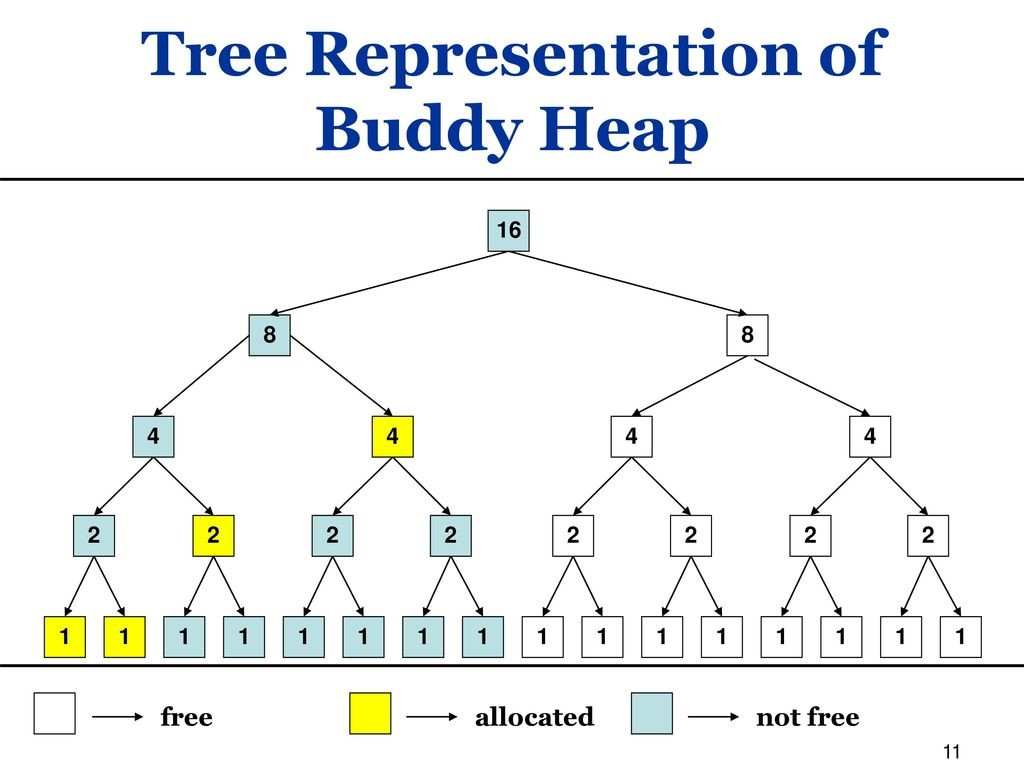
\includegraphics[scale=1.3]{imagens/BuddyHeap.jpg}
   \caption{Divisão da memória usando \emph{BuddyHeap}.\cite{arleen2018}}
   \label{fig:BuddyHeap}
\end{figure} 

O alocador \emph{kmalloc} é utilizado para solicitações de tamanho arbitrário. Assim o serviço aloca páginas inteiras sob demanda e, em seguida, divide-as em pedaços menores para satisfazer as requisições frequentes de pequenos blocos de memória. A alocação de memória utilizando esse serviço envolve determinar uma lista, entre as listas mantidas pelo \emph{kernel} das páginas alocadas, utilizando o primeiro bloco disponível na lista ou alocando uma nova página e subdividindo-a.\\ O \emph{kmalloc} não tem permissão e ou autoridade para relocar ou liberar regiões de memória já alocados mesmo que seja esta uma tratativa para uma possível falta de memória, depois de alocadas, essas regiões somente poderão ser reutilizadas mediante uma liberação explicita. Outros três subsistemas principais que tratam de sua própria gerência de páginas físicas e que interagem intimamente entre si, segundo Silberschatz(2000) são o \emph{cache} de \emph{buffers}, que é o \emph{cache} principal do \emph{kernel} para dispositivos orientados a bloco; o \emph{cache} de páginas que mantém em \emph{cache} páginas inteiras de conteúdo de arquivos, dados da rede entre outros e o sistema de memória virtual que gerencia o espaço de endereçamento virtual de cada processo \cite{Tanenbaum2016}, \cite{ufscar2019}, \cite{silberschatz2000}, \cite{stallings2004}.

\section{Memória Virtual}

O sistema de memória virtual no \emph{Linux} é responsável pela manutenção do espaço de endereçamento visível para cada processo assim sendo a criação das páginas de memória virtual sob demanda e a gerência do carregamento dessas páginas para o disco, ou o descarregamento de volta para o disco, é responsabilidade desse sistema.\\
O gerente de memória virtual mantem duas perspectivas do espaço de endereçamento de um processo sendo a primeira, é a visão lógica e a segunda a visão física de cada espaço de endereçamento \cite{ufscar2019}, \cite{silberschatz2000}, \cite{stallings2004}.\\
Na primeira instruções recebidas pelo sistema de memória virtual referentes  ao layout do espaço de endereçamento que consiste em um conjunto de regiões não superpostas, com cada uma representando um subconjunto contínuo e alinhado por página do espaço de endereçamento e sendo descrita internamente por uma única estrutura \emph{vm\_area \_struct} (é uma estrutura de dados utilizada para descrever uma área da memória virtual para um processo), que define as propriedades da região. Na segunda é armazenada uma tabela de páginas do \emph{hardware} para o processo e é gerenciada por um conjunto de rotinas.\\
 Cada \emph{vm\_area \_struct}  na descrição do espaço de endereçamento contém um campo que aponta para uma tabela de funções que implementam as funções básicas de gerência de página para qualquer região dada da memória virtual \cite{ufscar2019}, \cite{silberschatz2000}, \cite{stallings2004}.\\
No \emph{Linux} existem diversos tipos de região de memória virtual mais suas propriedades de caracterização são do tipo de armazenamento secundário associado e sua reação a escritas, as regiões de espaço de endereçamento de um processo pode ser privada ou compartilhada sendo feito um processo \emph{Copy-on-write} (é a operação onde uma região privada é copiada para uma nova região a fim de preservar essa região contra escritas a partir de outro processo) quando tentar escrever em uma região privada de outro processo, copiando o conteúdo da região para uma outra região nova e efetua as alterações na região recém-criada, preservando a região privada. Caso está escrita seja feita em região compartilhada o objeto mapeado para tal região é atualizado, de modo que as alterações ficam visíveis de imediato para todos os processos que estiverem mapeando tal objeto.\\
O \emph{Linux} cria espaços de endereçamento através de duas situações em um novo programa que é chamado solicitando ao sistema de execução um novo espaço de endereçamento, no qual o processo ao receber este espaço ele está completamente vazio, e a rotina carrega o programa para ocupar o espaço, ou quando um novo processo é criado por \emph{fork}, o que significa que uma cópia completa do espaço de endereço é criada para o processo existente \cite{ufscar2019}, \cite{silberschatz2000}, \cite{stallings2004}.


\section{Swapping e paginação}

Com uma crescente utilização da memória através de sistemas de tempo compartilhado ou computadores pessoais orientados graficamente por vezes a memória principal não possuem espaço suficiente para manter todos os processos ativos uma solução para isso é salvar parte destes processos excedentes colocando os no disco liberando assim espaço para novos processos e estes ficando em stand-by esperando serem chamados novamente. Assim sendo dependendo do \emph{hardware} duas técnicas podem ser utilizadas \cite{ufscar2019}, \cite{silberschatz2000}, \cite{stallings2004}.\\
A técnica mais simples, é o /emph{swapping} usada para algoritmos de escalonamento, baseando-se em prioridades. Se um processo de prioridade mais alta necessitar ser carregado, o gerenciador de memória poderá descarregar um outro com prioridade mais baixa para o disco, para que o de maior prioridade possa ser executado. Quando for finalizado, o processo descarregado pode então, ser carregado novamente para a memória principal. Segundo Silberschatz(2000), quando o escalonador de CPU executar um processo, ele chama o \emph{dispatcher} (também chamado de agendador de curto prazo, conforme Stallings(2004) descreve, decide qual dos processos na memória, prontos para a execução, será executado pelo processador) , que verifica se o próximo processo na fila está na memória. Se o processo não estiver na memória e não houver região de memória livre, o \emph{dispatcher} descarrega um processo que está na memória \emph{(swap out)} e carrega o processo desejado em seu lugar \emph{(swap in)}, recarregando, então, os registradores de forma usual e transferindo o controle para o processo selecionado \cite{ufscar2019}, \cite{silberschatz2000}, \cite{stallings2004}.\\
No \emph{Linux}, o processo de paginação pode ser dividido em duas seções: o algoritmo de políticas, primeiramente, que decide que páginas são gravadas no disco e quando esse processo será feito, por meio de uma versão modificada do algoritmo de relógio, que emprega um relógio de passagens múltiplas. \\
A segunda seção, é o mecanismo de paginação, que suporta tanto partições e dispositivos dedicados, quanto arquivos, sendo que no último, o processo pode ser mais lento devido ao custo adicional provocado pelo sistema de arquivos. O algoritmo utilizado para a gravação das páginas é o algoritmo \emph{next-fit}, para tentar gravar páginas em carreiras contínuas de blocos de disco, visando um melhor desempenho \cite{ufscar2019}, \cite{silberschatz2000}, \cite{stallings2004}.

\chapter{Sistemas de arquivos}\label{cap:SistemasArquivos}

Arquivos são unidades lógicas de informação criadas por processos. Podemos pensar nos arquivos como espaços de endereçamento que são usados para modelar o disco em vez da memória \emph{RAM} os processos podem ler estes e através dos dados contidos neles gerar novos caso necessário. As informações contidas nos arquivos devem ser persistentes, ou seja, mesmo após o termino do processo elas devem ser mantidas integras para utilização futura exceto quando o próprio utilizador do sistema deseja excluir este. No \emph{Linux} os arquivos sofrem uma estrutura hierárquica onde podemos ter níveis de permissões variando entre proprietário, grupo ao qual o proprietário pertence e público (ou seja, qualquer usuário do sistema). Os arquivos normalmente possuem três operações básicas escrita, leitura e execução \cite{Morimoto2011}, \cite{guialinux2020}, \cite{luciano2015}.\\
Arquivos são gerenciados pelo sistema operacional. Como são estruturados, nomeados, acessados, usados, protegidos, implementados e gerenciados são tópicos importantes no projeto de um sistema operacional. Como um todo, aquela parte do sistema operacional lidando com arquivos é conhecida como sistema de arquivos.\\
Basicamente o sistema de arquivos é um conjunto de estruturas logicas que permite o sistema operacional controlar o acesso a um dispositivo de armazenamento, diferentes sistemas operacionais podem usam diferentes sistemas de arquivos, atualmente, o \emph{NTFS (New Technology File System)} é o sistema de arquivos padrão do \emph{Windows}, enquanto o \emph{ext4} é o do \emph{Linux} \cite{Morimoto2011}, \cite{guialinux2020}, \cite{luciano2015}.\\
\\Abaixo podemos ver alguns dos sistemas de arquivos mais conhecidos:\\
\\•	\emph{EXT3 (third extended filesystem)} – foi adotado como padrão \emph{Linux} a partir de 2001. Introduziu o registro \emph{(journal)} que melhora a confiabilidade e permite recuperar o sistema em caso de desligamento não programado. \emph{EXT3} suporta 16TB (1 terabyte corresponde a 240 bytes) de tamanho máximo no sistema de arquivos, e 2TB de tamanho máximo de um arquivo. Um diretório pode ter, no máximo, 32.000 subdiretórios.\\
\\•	\emph{EXT4 (fourth extended filesystem)} – passou a ser o padrão \emph{Linux} a partir de 2008. \emph{EXT4} suporta 1EB (1 exabyte corresponde a 260 bytes) de tamanho máximo de sistema de arquivos e 16TB de tamanho máximo de arquivos. É possível ter um número ilimitado de subdiretórios.\\
\\•	\emph{XFS (Extended Filesystem)} – usado como padrão por algumas distribuições \emph{Linux} desde 2014. \emph{XFS} é um sistema de arquivos desenvolvido em 64 bits, compatível com sistemas de 32 bits. Ele suporta até 16 EB de tamanho total do sistema de arquivos e até 8 EB de tamanho máximo para um arquivo individual. É considerado um sistema de arquivos de alto desempenho.\\
\\•	\emph{JFS (Journaled File System)} – é um sistema de arquivos de 64 bits com \emph{journaling} desenvolvido pela \emph{IBM}.\\
\\•	\emph{HFS (Hierarchical File System)} – é um sistema de arquivos proprietário da \emph{Apple}.\\
    \\•	\emph{FAT (File Allocation Table)} – é um sistema desenvolvido para o \emph{MS-DOS} e usado em versões do \emph{Microsoft Windows} até o \emph{Windows 95}. É suportado praticamente por todos os sistemas operacionais existentes. Existem 3 versões do sistema: \emph{FAT} (12 bits, usado pelos disquetes), \emph{FAT16} (para OS 16 bits ou 32 bits) e \emph{FAT32} (só para SO a 32 bits).\\
\\•	\emph{NTFS (New Technology File System)} é o sistema de arquivos padrão do sistema operacional \emph{Microsoft Windows}. São algumas características deste tipo de sistema: aceita volumes de até 2 TB; o tamanho do arquivo é limitado apenas pelo tamanho do volume; é um sistema de arquivos muito mais seguro que o \emph{FAT}; \emph{NTFS }podem se recuperar de um erro mais facilmente.\\
\\•	\emph{HPFS} –  é o sistema de arquivos utilizado pelo \emph{OS/2} da \emph{IBM}, com recursos que se aproximam muito dos permitidos pelo \emph{NTFS}.\\
\\•	\emph{UFS (Unix File System)} – é um sistema de arquivos usados por muitos sistemas operacionais \emph{Unix} e assemelhados \cite{Morimoto2011}, \cite{guialinux2020}, \cite{luciano2015}.\\

\section{Gerenciamento de diretório}

Sistemas de arquivos normalmente têm diretórios ou pastas, que podem ser de nível único ou hierárquicos.\\
Segundo Tanenbaum(2016) a forma mais simples de um sistema de diretório é ter um diretório contendo todos os arquivos. Às vezes ele é chamado de diretório-raiz. \\Essa decisão foi tomada sem dúvida para manter simples o \emph{design} do \emph{software}. Um exemplo de um sistema com um diretório é dado na Figura \ref{fig:DiretorioRaiz}. Aqui o diretório contém quatro arquivos. As vantagens desse esquema são a sua simplicidade e a capacidade de localizar arquivos rapidamente às vezes ele ainda é usado em dispositivos embarcados simples como câmeras digitais e alguns \emph{players} portáteis de música \cite{Tanenbaum2016}. \\\\

\begin{figure}[htpb]
    \centering
   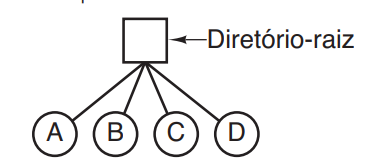
\includegraphics[scale=1]{imagens/DiretorioRaiz.png}
   \caption{Um sistema de diretório em nível único contendo
   quatro arquivos. \cite{Tanenbaum2016}}
   \label{fig:DiretorioRaiz}
\end{figure} 

Apesar do método anterior ser mais simples em atualmente os usuários em seus dispositivos milhares de arquivos inviabilizando o modelo anterior em consequência, é necessária uma maneira para agrupar arquivos relacionados em um mesmo local\cite{Tanenbaum2016}. 
Faz-se necessária uma hierarquia (isto é, uma árvore de diretórios). Com essa abordagem, o usuário pode ter tantos diretórios quantos forem necessários para agrupar seus arquivos de maneira natural. 
Além disso, se múltiplos usuários compartilham um servidor de arquivos comum, como é o caso em muitas redes de empresas, cada usuário pode ter um diretório-raiz privado para sua própria hierarquia. Essa abordagem é mostrada na Figura \ref{fig:DiretorioRaiz2} \cite{Tanenbaum2016}. 

\begin{figure}[htpb]
    \centering
   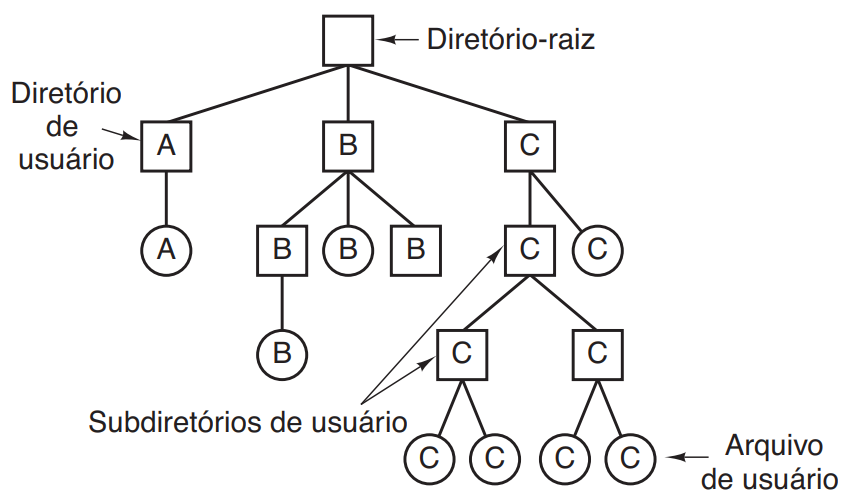
\includegraphics[scale=0.7]{imagens/DiretorioRaiz2.png}
   \caption{Um sistema hierárquico de diretórios. \cite{Tanenbaum2016}}
   \label{fig:DiretorioRaiz2}
\end{figure} 

No \emph{Linux} o diretório raiz e o diretório “/” é o diretório com maior hierarquia entre todos os diretórios do sistema assim todos os outros diretórios estão abaixo dele\cite{Morimoto2011}, \cite{guialinux2020}, \cite{luciano2015}.\\ \\
\\A seguir são apresentados exemplos de diretórios que normalmente ficam abaixo do diretório raiz.\\
•	bin – diretório com os comandos disponíveis para os usuários comuns (não privilegiados).\\
•	boot – diretório com os arquivos estáticos do \emph{boot} de inicialização.\\
•	dev – diretório com as definições dos dispositivos de entrada/saída.\\
•	etc – diretório com os arquivos de configuração do sistema.\\
•	home – diretório que armazena os diretórios dos usuários do sistema.\\
•	lib – diretório com as bibliotecas e módulos (carregáveis) do sistema.\\
•	lost+found – é usado pelo \emph{fsck} para armazenar arquivos/diretórios/devices corrompidos.\\
•	media – ponto de montagem temporário para mídias removíveis.\\
•	mnt – ponto de montagem temporário para sistemas de arquivos.\\
•	opt – \emph{softwares} adicionados pelos usuários.\\
•	proc – diretório com informações sobre os processos do sistema.\\
•	root – diretório \emph{home do root}.\\
•	run – armazena arquivos temporários da inicialização do sistema.\\
•	sbin – diretório com os aplicativos usados na administração do sistema.\\
•	snap – diretório com pacotes snaps (podem ser executados em diferentes distribuições \emph{Linux}).\\
•	srv – dados para serviços providos pelo sistema.\\
•	sys – contém informações sobre \emph{devices, drivers} e características do \emph{kernel}.\\
•	tmp – diretório com arquivos temporários.\\
•	usr – diretório com aplicativos e arquivos utilizados pelos usuários como, por exemplo, o sistema de janelas X, jogos, bibliotecas compartilhadas, programas de usuários e de administração, etc.\\
•	var – diretório com arquivos de dados variáveis (\emph{spool, logs}, etc).\\
\\Três comandos básicos do \emph{Linux server} para se deslocar entre diretórios são:\\
\\\emph{pwd (print working directory)}: informa o diretório de trabalho - ou corrente, apresentando o caminho desde o raiz até o diretório atual.\\
\\\emph{ls (list space)}: lista, de maneira simples ou com informações variadas, arquivos específicos ou o conteúdo de diretórios.\\
\\\emph{cd (change directory)}: serve para fazer a mudança entre os diretórios - como o próprio nome informa o seu uso pode ser para caminhar na pasta local, dentro da própria pasta, ou para qualquer local do sistema.\\
\\Compartilhamento de arquivos muitas vezes é necessário que um arquivo se mostre simultaneamente em diretórios diferentes por estar compartilhado entre vários usuários ou por possuir informação que são necessárias para o sistema como na figura \ref{fig:DiretorioRaiz3} abaixo \cite{Tanenbaum2016}: 

\begin{figure}[htpb]
    \centering
   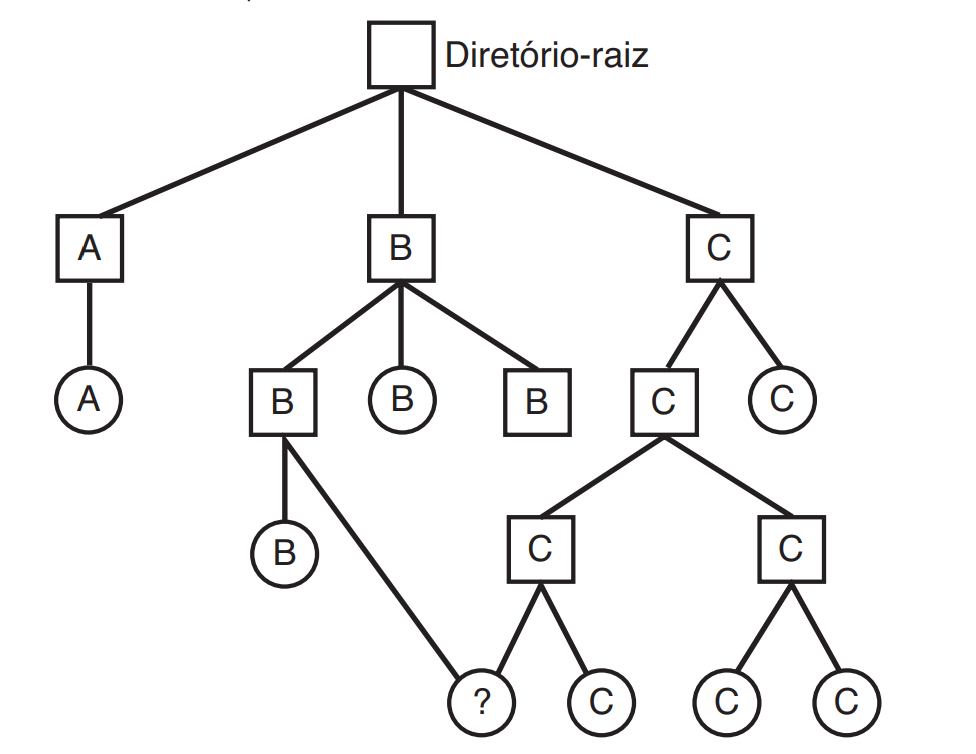
\includegraphics[scale=0.55]{imagens/DiretorioRaiz3.png}
   \caption{Sistema de arquivos contendo um arquivo
   compartilhado.  \cite{Tanenbaum2016}}
   \label{fig:DiretorioRaiz3}
\end{figure} 

O compartilhamento de arquivos pode gerar alguns problemas se os diretórios realmente contiverem endereços de disco, então uma cópia desses endereços terá de ser feita no diretório do de cada usuário quando o arquivo for utilizado subsequentemente se cada usuário adicionarem blocos de arquivos em seu diretório pessoal quando utilizarem o arquivo é praticamente como se o usuário estivesse copiando o arquivo para seu diretório assim perdendo o sentido do compartilhamento \cite{Tanenbaum2016}.\\
Segundo Tanenbaum(2016) ele diz que esse problema pode ser solucionado de duas maneiras. Na primeira solução, os blocos de disco não são listados em diretórios, mas em uma pequena estrutura de dados associada com o arquivo em si. Os diretórios apontariam então apenas para a pequena estrutura de dados. Essa é a abordagem usada em \emph{UNIX} (em que a pequena estrutura de dados é o \emph{i-node}).
A segunda solução seria que quando um novo usuário utilize do arquivo seja criado um arquivo \emph{link} que irá conter apenas uma receita do arquivo original contendo seu o caminho do arquivo que está sendo utilizado, essa abordagem é chamada de ligação simbólica \cite{Tanenbaum2016}.

\section{Gestão de espaço livre}

Arquivos são armazenados em disco e os discos possuem limites físicos quanto a tamanho do disco e quantidade de arquivos que podem ser armazenados. Visto isso o gerenciamento do espaço do disco é uma das preocupações do projetista de sistemas de arquivos \cite{Tanenbaum2016}. \\
O primeiro consiste em usar uma lista encadeada de blocos de disco, com cada bloco contendo tantos números de blocos livres de disco quantos couberem nele. Com um bloco de 1 KB e um número de bloco de disco de 32 bits, cada bloco na lista livre contém os números de 255 blocos livres \cite{Tanenbaum2016}.\\
A outra técnica de gerenciamento de espaço livre é o mapa de bits. Um disco com n blocos exige um mapa de bits com n bits. Blocos livres são representados por 1s no mapa, blocos alocados por 0s (ou vice-versa) \cite{Tanenbaum2016}.\\ Para nosso disco de 1 TB de exemplo, precisamos de 1 bilhão de bits para o mapa, o que exige em torno de 130.000 blocos de 1 KB para armazenar \cite{Tanenbaum2016}.\\ Não surpreende que o mapa de bits exija menos espaço, tendo em vista que ele usa 1 bit por bloco, versus 32 bits no modelo de lista encadeada.  

\begin{figure}[htpb]
    \centering
   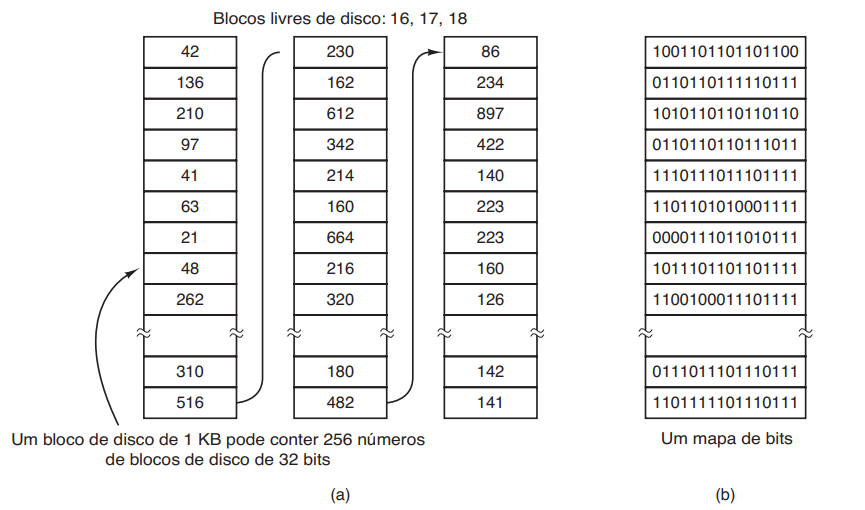
\includegraphics[scale=.8]{imagens/GestaoLivre.png}
   \caption{(a) Armazenamento da lista de blocos livres em uma lista encadeada. (b) Um mapa de bits. \cite{Tanenbaum2016}}
   \label{fig:GestaoLivre}
\end{figure} 

\section{Cotas de disco}

É comum em sistemas de multiusuários que os sistemas definam cotas de disco que é um mecanismo para impor um tamanho máximo de utilização para cada usuário assim ele impede que o usuário utilize o sistema de forma a prejudicar o funcionamento do sistema\cite{Tanenbaum2016}. \\. 
Quando um usuário abre um arquivo é gerada uma tabela de arquivos aberta na memória principal com os atributos endereços de disco são localizados. Quaisquer aumentos no tamanho do arquivo serão cobrados da cota do proprietário, uma segunda tabela é contendo os registros de cotas de todos os usuários com um arquivo aberto, mesmo que esse arquivo tenha sido aberto por outra pessoa. Essa tabela está mostrada na Figura \ref{fig:CotaDisco}. Ela foi extraída de um arquivo de cotas no disco para os usuários cujos arquivos estão atualmente abertos. Quando todos os arquivos são fechados, o registro é escrito de volta para o arquivo de cotas. Quando uma nova entrada é feita na tabela de arquivos abertos, um ponteiro para o registro de cota do proprietário é atribuído a ela, a fim de facilitar encontrar os vários limites \cite{Tanenbaum2016}. \\
Toda vez que um bloco é adicionado a um arquivo, o número total de blocos cobrados do proprietário é incrementado, e os limites flexíveis e estritos são verificados. O limite flexível pode ser excedido, mas o limite estrito não. Esse método tem a propriedade de que os usuários podem ir além de seus limites flexíveis durante uma sessão de uso, desde que removam o excesso antes de se desconectarem. Os limites estritos jamais podem ser excedidos \cite{Tanenbaum2016}.

\begin{figure}[htpb]
    \centering
   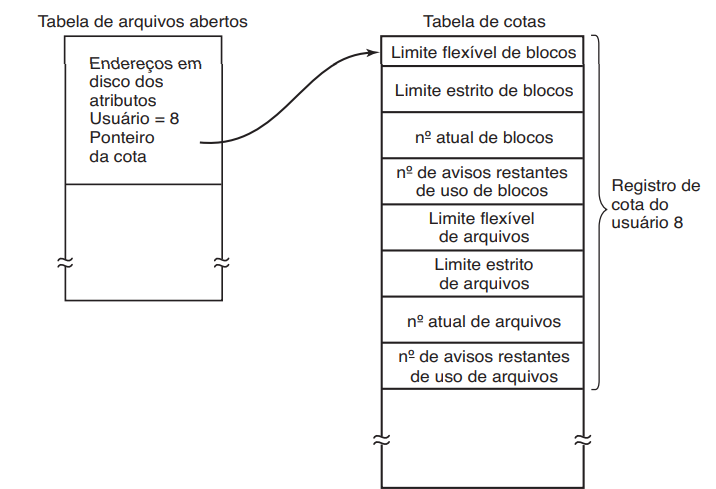
\includegraphics[scale=0.6]{imagens/CotaDisco.png}
   \caption{As cotas são relacionadas aos usuários e monitoradas em uma tabela de cotas. \cite{Tanenbaum2016}}
   \label{fig:CotaDisco}
\end{figure} 

% PARTE - Define a divisão do documento em partes (Não é obrigatório)
%\part{Preparação da pesquisa}
%% ---
\chapter{Uso de referências bibliográficas}
% ---

A formatação das referências bibliográficas conforme as regras da ABNT são um
dos principais objetivos do \abnTeX. Consulte os manuais
\citeonline{abntex2cite} e \citeonline{abntex2cite-alf} para obter informações
sobre como utilizar as referências bibliográficas.

%-
\subsection{Acentuação de referências bibliográficas}
%-

Normalmente não há problemas em usar caracteres acentuados em arquivos
bibliográficos (\texttt{*.bib}). Porém, como as regras da ABNT fazem uso quase
abusivo da conversão para letras maiúsculas, é preciso observar o modo como se
escreve os nomes dos autores. Na~\autoref{tabela-acentos} você encontra alguns
exemplos das conversões mais importantes. Preste atenção especial para `ç' e `í'
que devem estar envoltos em chaves. A regra geral é sempre usar a acentuação
neste modo quando houver conversão para letras maiúsculas.

\begin{table}[htbp]
\caption{Tabela de conversão de acentuação.}
\label{tabela-acentos}

\begin{center}
\begin{tabular}{ll}\hline\hline
acento & \textsf{bibtex}\\
à á ã & \verb+\`a+ \verb+\'a+ \verb+\~a+\\
í & \verb+{\'\i}+\\
ç & \verb+{\c c}+\\
\hline\hline
\end{tabular}
\end{center}
\end{table}


% ---
\section{Precisa de ajuda?}
% ---

Consulte a FAQ com perguntas frequentes e comuns no portal do \abnTeX:
\url{https://code.google.com/p/abntex2/wiki/FAQ}.

Inscreva-se no grupo de usuários \LaTeX:
\url{http://groups.google.com/group/latex-br}, tire suas dúvidas e ajude
outros usuários.



%\chapter{Estado da Arte}\label{cap:estArte}

\lipsum[34]

\section*{Trabalhos Relacionados a Isto}\label{sec:primTrab}
\addcontentsline{toc}{section}{Trabalhos Relacionados a Isto}

\lipsum[34-36]
%\chapter{Materiais e Métodos}\label{cap:ferramentas}

\lipsum[43-45]

\section{Considerações Finais}

\lipsum[23]


% PARTE
%\part{Proposta}
%\chapter{Sistema Proposto}\label{cap:proposta}

Esse trabalho propõe um sistema de... 


\section{Primeira Parte do Sistema Proposto}

\lipsum[67]

\section{Considerações Finais}

\lipsum[68]


% PARTE
%\part{Parte Final}
%\chapter{Resultados e Discussão}\label{cap:resultados}

\lipsum[73]

\section{Base de Dados}

\lipsum[72]

\section{Considerações Finais}

\lipsum[74]
\chapter*{Conclusão}\label{cap:conclusao}
\addcontentsline{toc}{chapter}{Conclusão}

Durante este estudo foi possível compreender a gigantesca extensão das atividades de um Sistema operacional, com o desenvolvimento do estudo este modelo expos o sistema e tudo o que ele gerencia. \\
Foram vistos todas as estruturas seja de /emph{hardware} ou /emph{Software} que o sistema operacional se utiliza ou gerencia para prover uma abstração para o usuário de forma a ser uma utilização transparente em especial o /emph{Linux} por ser um /emph{Software Livre} implica, por definição, na abertura da possibilidade de se deter todo o conhecimento embutido em uma aplicação. A tecnologia de sistemas de informação deixa de ser uma 'caixa preta' criada por uma 'sociedade superior', passando a estar ao alcance de todos.
Outro fator importante apresentado foi a importância dos sistemas na utilização dos recursos computacionais.\\
Por fim, foi visto no decorrer do trabalho que os sistemas operacionais são de fundamental base de utilização para a área da tecnologia representando uma área de conhecimento que tem muito a agregar para todos aqueles envolvidos com ambientes computacionais.

% \section*{Conclusões}
% \section*{Trabalhos Futuros}

% ----------------------------------------------------------
% ELEMENTOS PÓS-TEXTUAIS (Referências, Glossário, Apêndices)
% ----------------------------------------------------------
\postextual

% Referências bibliográficas
\bibliography{bibliografia}
\bibliographystyle{IEEEtran}
% Glossário (Consulte o manual)
%\glossary

% Apêndices
%% ----------------------------------------------------------
% Apêndices
% ----------------------------------------------------------

% ---
% Inicia os apêndices
% ---
\begin{apendicesenv}

% Imprime uma página indicando o início dos apêndices
\partapendices

% ----------------------------------------------------------
\chapter{Primeiro Apêncice}
% ----------------------------------------------------------

\lipsum[50] % Texto qualquer. REMOVER!!

% ----------------------------------------------------------
\chapter{Perceba que o texto do título desse segundo apêndice é bem grande}
% ----------------------------------------------------------
\lipsum[51-53] % Texto qualquer. REMOVER!!

\end{apendicesenv}
% ---

% Anexos
%% ----------------------------------------------------------
% Apêndices
% ----------------------------------------------------------

% ---
% Inicia os anexos
% ---
\begin{anexosenv}

% Imprime uma página indicando o início dos anexos
\partanexos

% ---
\chapter{Nome do Primeiro Anexo}
% ---
\lipsum[30] % Texto qualquer. REMOVER!!

% ---
\chapter{Nome de Outro Anexo}
% ---

\lipsum[32] % Texto qualquer. REMOVER!!

\end{anexosenv}

% Índice remissivo (Consultar manual)
%\phantompart
%\printindex

\end{document}
